\subsection{Layer-Wise Relevance Decomposition}
\begin{figure*}
    \center
    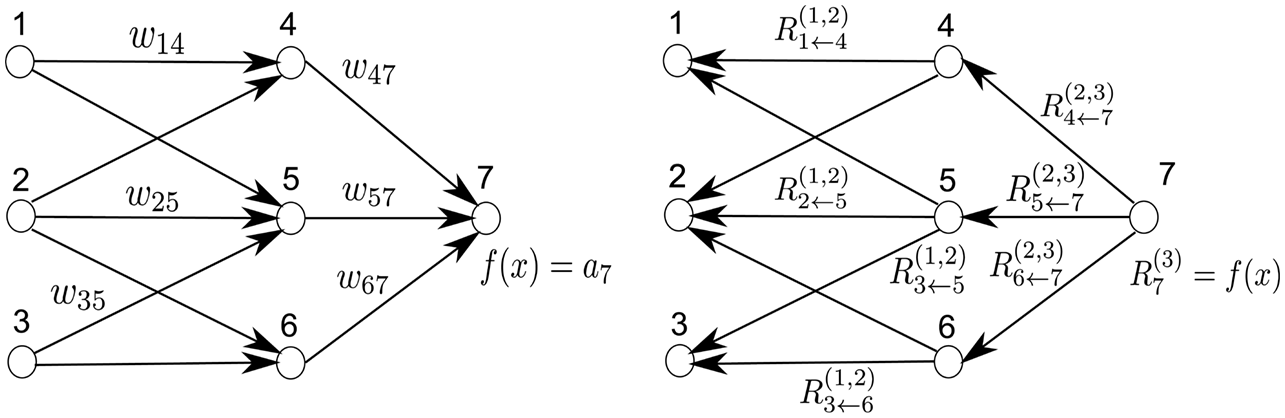
\includegraphics[]{lrp-fig2.PNG}
    \caption{\textbf{Left:} A neural network at prediction time. \textbf{Right:} a neural network at relevance-propagation time, adopted from \protect\cite{Bach.2015}}\label{fig:lrp-nn}
\end{figure*}
\gls{lrp} attempts to provide a measure for the \nameref{subsubsect:pixel-wise-decomp}, discussed earlier in \cref{subsubsect:pixel-wise-decomp}. The relevances are computed \textit{backwards} from the output of the model (\(f(x)\)) to its input (\(x\)) after prediction time. Relevance is denoted as \(R_{i}^{l}\), the relevance of neuron \(i\) in layer \(l\), where \(l=1\) is the input layer. \gls{lrp} is formulated by \fcite{Bach.2015} as a set of constraints:
\begin{itemize}
    \item \gls{lrp} must follow \ref{subsubsect:pixel-wise-decomp} completely.
    \item each layer of the neural network can be represented by relevances, such that 
    \begin{multline}
        f(x) = \dots \\ 
        = \sum_{j\in l+1} R_j^{(l+1)} = \sum_{i\in l} R_i^{(l)} \\
        = \dots = \sum_{h\in x} R_h^{(1)}.\label{eq:lw-propagation}
    \end{multline}
    Informally, \cref{eq:lw-propagation} implies that relevances can be propagated from the predictor-output \(f(x)\) to the input-variables in \(x\).
    \item the relevance of the \textit{output neuron} is defined as the model-output \(f(x)\)
    \item the relevance of \textit{every other neuron} is the sum of its incoming \glspl{message}, formally 
    \begin{equation}
        R_i^{(l)} = \sum_{\left\{ j | \text{Path } P_{i \rightarrow j} \text{ exists}\right\}} R_{i\leftarrow j}^{(l, l+1)}\label{eq:incoming-messages}
    \end{equation}
    \item the total relevance that a neuron sends out as \glspl{message} is equal to its own relevance, formally
    \begin{equation}
        R_j^{(l+1)} = \sum_{\left\{ i | \text{Path } P_{i \rightarrow j} \text{ exists}\right\}} R_{i\leftarrow j}^{(l, l+1)}
    \end{equation}
    \item each \gls{message} \(R_{i\leftarrow j}^{(l,l+1)}\) is the product of the relevance of neuron \(j\), \(R_j^{(l+1)}\), weighted by the \textit{relative strength} of the path \(P_{i\rightarrow j}\), formally
    \begin{equation}
        R_{i\leftarrow j}^{(l,l+1)} = R_{j}^{(l+1)} \frac{a_i w_{ij}}{\sum_h a_h w_{hj}},
    \end{equation}
    where \(a_i\) is the output of neuron \(i\) (precisely the output of its activation-function) and \(w_ij\) are the weights that connect neurons \(i \text{ and } j\)
\end{itemize}
In summary, \gls{lrp} requires a conservation of relevance between layers, the relevance of a neuron to be the sum of its incoming weighted \glspl{message} and also its outgoing weighted \glspl{message} \todo{turn itemize into list and reference the points in the summary accordingly. that would be nice}

\subsubsection{Taylor-Decomposition}
\blindtext[1]

\subsubsection{Deep-Taylor-Decomposition}
\blindtext[1]